\subsection{Synchronization problem}
This design does have one major problem with synchronization.
It can never be decided in an asynchronous communication model
if the other node will ever respond and when it will respond.
The proposed block by A only needs an interaction of B to be finished
and B can finish this transaction at anytime that B decides upon.

But the future block contains an immutable hash pointer
to the previous block in the chain of node A.
So while this transaction for a potential block is outstanding,
node A cannot interact with any other node C to create a different block.
If it would, then B could ultimately respond and a branch with different blocks
would be created for the chain of A.
This simple design introduces therefor an external response dependency problem.

The to-be-designed system has to be fault tolerant to
common problems in a challenged network, such as node failure.
A second design goal is to be able to process transactions quickly and on a large scale.
These design goals prevent the adaption of a simple design that will halt until node B responds.
This design would also result in a deadlock situation, as explained in section \ref{sect:deadlock}
We will explain three possible design solutions to this problem.

\subsubsection{Fair exchange signature scheme}
A fair exchange signature scheme~(FESS) allows two players to exchange digital signatures in a fair way.
Fair constitutes that no player can take advantage of the other.
Either both players receive each others signature or no player receives the other's signature.
It is infeasible for a node to acquire a signature without giving up their own signature~\cite{asokan-fairexchange},
a FESS could be implement for the fair creation of the block.

But currently all known FESSs use a trusted third party (TTP) at some point~\cite{asokan-fairexchange}.
Some schemes exist that are optimistic and will only need a TTP to resolve conflicts.
But any TTP will not adhere to the Tribler philosophy
of being a truly fully distributed peer-to-peer system.
The TTP will introduce a central point of trust and a scalability bottleneck.

\subsubsection{Reverse repairing of chain}
Another potential solution would be to rework part of the chain.
The creation of block could be deemed to have failed by node A.
If at a later point the block is still created by B,
then the block could be reworked back into the chain.
This would require every hash pointer to be updated afterwards.
If these hash pointers are modified, then the signatures are invalid.
Every signature would have to be renewed and requested at every node.
This is unscalable if nodes needs to rework many blocks and can clog the system.
These nodes can possibly no longer respond and would result in new invalid blocks.

\subsubsection{Half signed blocks}
\label{des:halfsigned}
The chosen solution is to keep it simple and allow for inconsistencies between the chains of A and B.
It will be shown that when an inconsistency does occur, this is in favor of A.

When node A sends a signature request to B,
then A will be optimistic and will wait for B for a timeout period.
During this time, A will not interact with another node C.
But if A does not have to interact with node C after the timeout period,
then A will keepw waiting for a response of B and accept the response.
There are three potential scenario's of what will happen to the message.

\begin{enumerate}
\item
In the normal situation, node B will respond in time to the message.
B will send back the message
and both A and B will have added the same block in their own chains.
This situation also occurs if A has timed out,
but has not yet interacted with another node C.

\item
Node B can be malicious or simply have failed and B will never respond.
Node A will timeout, add a half signed block to the chain and can continue interacting with other nodes C.
A will have to decide how to react upon B not responding.
A possibility would be to stop helping B.

\item
The response of B can also be late.
After B has received the request by A,
B will create a block and adds this block to its chain.
B will send its response to A,
but the message will arrive too late at A.
A will have experienced a timeout and  will ignore the message.
The block is not added to the chain of A.
\end{enumerate}

The last scenario is the most complex and requires additional clarification.
A initiates the signature request as a seeder and therefore the block will be favourable for its reputation.
Because this is a reputation system, this inconsistency is an allowable comprimise.
In a currency system, this comprimise would not be allowable.

The design is scalable as it will not force a node to wait too long for a failed node
and will try to interact as fast as possible with other nodes.
A small grace period can be used to allow node B to have enough time to respond in a normal manner.
No trusted third party is introduced so a distributed design is achieved.

The contents of a half signed block can be seen in Figure \ref{fig:halfsigned-block}.
The total up, total down, previous hash, sequence number and signature of B are empty in an half signed block.
These are normally filled in by B and A does not have knowledge of these fields.

\begin{figure}
	\centerline{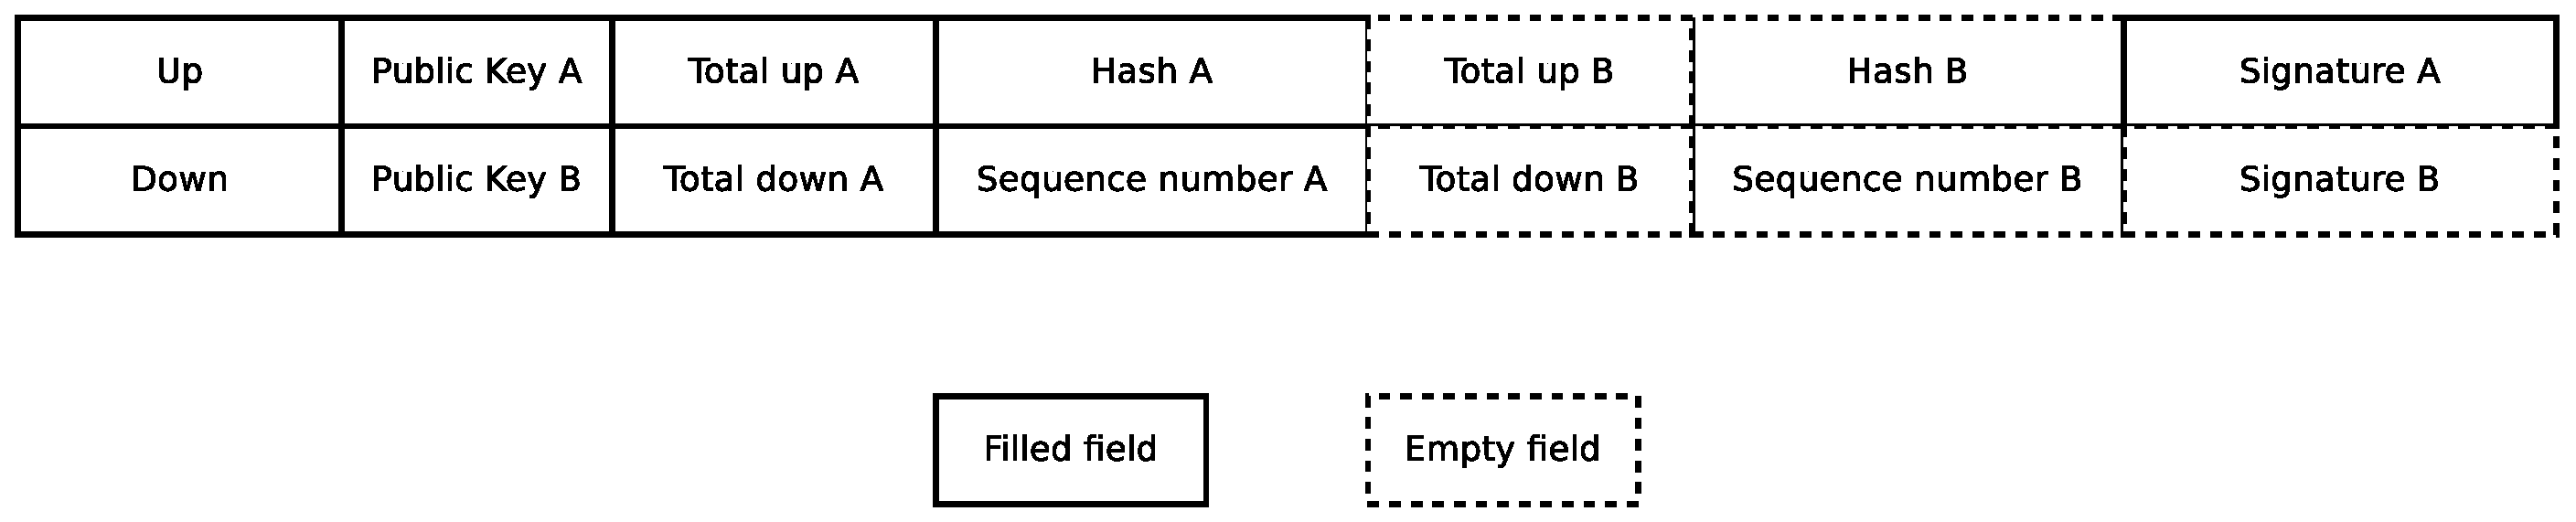
\includegraphics[scale=0.3]{design/figs/halfsigned-block.eps}}
	\caption{The fields of a half signed block in MultiChain. Dotted fields are empty.}
	\label{fig:halfsigned-block}
\end{figure}

An example of the chain with an half signed block can be seen in Figure \ref{fig:halfsigned-chain}.
In this example peer A initiates two block creations with B.
The second block response does not arrive on time at A and A has timed out.
The block cannot be processed as A has already interacted with C.
The half signed block is never referenced again by A.
B does continue using this block.
This is not double spending because A does not reuse the same previous hash.
The difference in block is only the addition of the data of B.
This changes the hash of the block and is why B and A have a different hash.

\begin{figure}
	\centerline{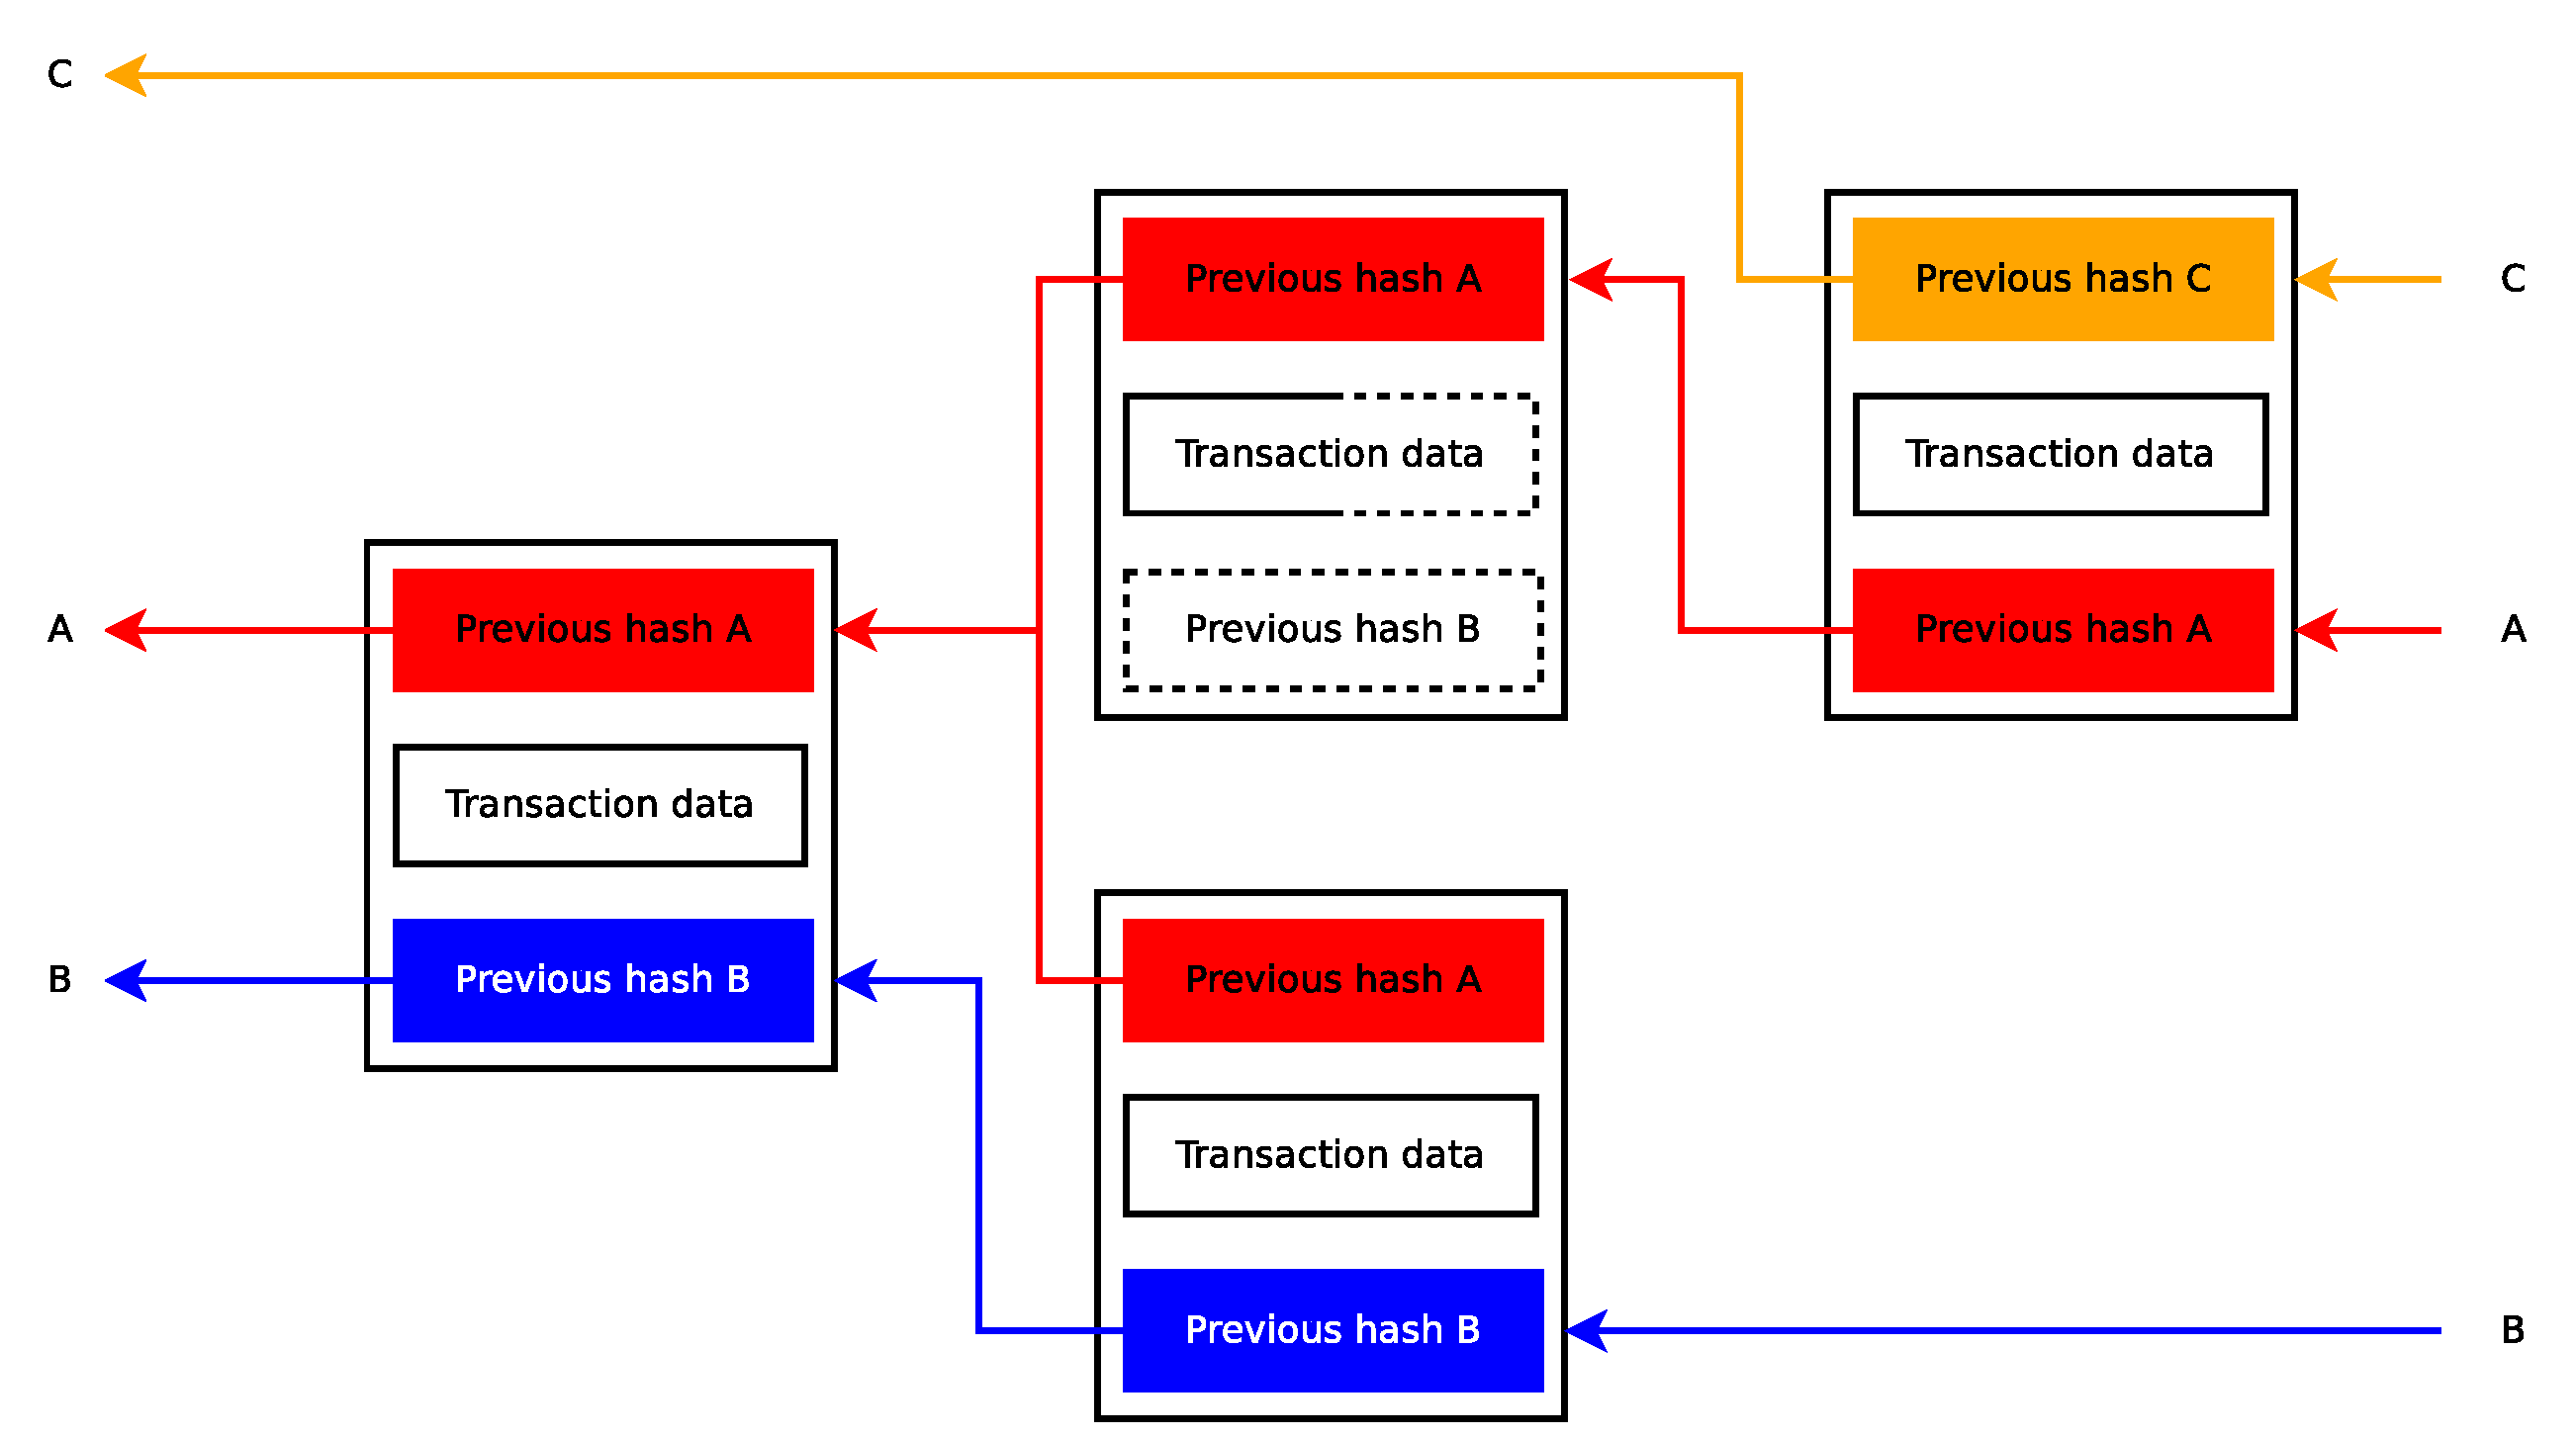
\includegraphics[scale=0.3]{design/figs/halfsigned-chain.eps}}
	\caption{A chain of with a half signed block in MultiChain.}
	\label{fig:halfsigned-chain}
\end{figure}

